\documentclass{article}%
\usepackage[T1]{fontenc}%
\usepackage[utf8]{inputenc}%
\usepackage{lmodern}%
\usepackage{textcomp}%
\usepackage{lastpage}%
\usepackage{geometry}%
\geometry{left=2.5cm,top=1.5cm}%
\usepackage[dvipsnames]{xcolor}%
\usepackage{tcolorbox}%
\usepackage{caption}%
\usepackage{array}%
%
%
%
\begin{document}%
\normalsize%
\section{Análisis Sísmico}%
\label{sec:AnlisisSsmico}%
\subsubsection{Irregularidad por Esquinas Entrantes}%
\label{ssubsec:IrregularidadporEsquinasEntrantes}%
\begin{tcolorbox}[colback=gray!5!white,colframe=cyan!75!black,fonttitle=\bfseries,title=Tabla N°9 E-030]%
\textit{La estructura se califica como irregular cuando los diafragmas tienen discontinuidades abruptas o variaciones importantes en rigidez, incluyendo aberturas mayores que 50\% del área bruta del diafragma.} \\ \textit{También  existe  irregularidad  cuando,  en  cualquiera de  los pisos y para cualquiera de las direcciones de análisis, se tiene alguna sección transversal del diafragma con un área neta resistente menor que 25\% del área de la sección transversal total de la misma dirección calculada con las dimensiones totales de la planta.}%
\end{tcolorbox}%


\begin{figure}[ht!]%
\centering%
\caption{Irregularidad por discontinuidad del diafragma}%
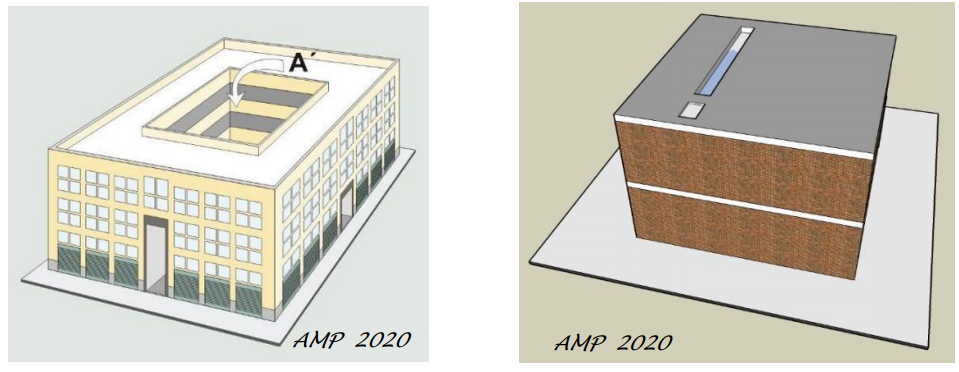
\includegraphics[scale=0.7]{i_diafragma.PNG}%
\caption*{\small Fuente: Muñoz (2020)}%
\end{figure}

%


\begin{table}[ht!]%
\centering%
\caption{Irregularidad por discontinuidad del diafragma (a)}%
\begin{tabular}{|ll|c|r}%
\cline{1-3}%
\multicolumn{2}{|l|}{Longitud del aligerado (L1)} & 7.51 & \multicolumn{1}{l}{m} \\%
\cline{1-3}%
\multicolumn{2}{|l|}{Espesor del aligerado (e1)} & 0.05 & \multicolumn{1}{l}{m} \\%
\cline{1-3}%
\multicolumn{2}{|l|}{Area del aligerado A1=L1$\cdot$ e1} & 0.38 & \multicolumn{1}{l}{$m^2$} \\%
\cline{1-3}%
\multicolumn{2}{|l|}{Longitud de la losa macisa (L2)} & 2.25 & \multicolumn{1}{l}{m} \\%
\cline{1-3}%
\multicolumn{2}{|l|}{Espesor de la losa macisa (e2)} & 0.2 & \multicolumn{1}{l}{m} \\%
\cline{1-3}%
\multicolumn{2}{|l|}{Area de la losa macisa A1=L1$\cdot$ e1} & 0.45 & \multicolumn{1}{l}{$m^2$} \\%
\cline{1-3}%
\multicolumn{2}{|l|}{Ratio} & 118.42 & \multicolumn{1}{l}{\%} \\%
\cline{1-3}%
\multicolumn{2}{|l|}{Ratio límite} & 25.00 & \multicolumn{1}{l}{\%} \\%
\cline{1-3}%
\multicolumn{2}{|l|}{Verificación} & \textcolor[rgb]{ .267,  .447,  .769}{\textbf{Regular}} & \multicolumn{1}{l}{} \\%
\cline{1-3}%
\end{tabular}%
\end{table}

%
\end{document}